\documentclass[tikz,border=2pt]{standalone}
\usepackage{amsmath}
\usepackage{pgfplots}
\pgfplotsset{compat=1.18}
\begin{document}
% x_t = x* + a^t (x_0 - x*) with x* = 6, x_0 = 10: a = 0.5 (x_{t+1} = 0.5x_t + 3) gives the monotone path
% 6 + 4(0.5)^t; a = -0.5 (x_{t+1} = -0.5x_t + 9) gives the alternating path 6 + 4(-0.5)^t.
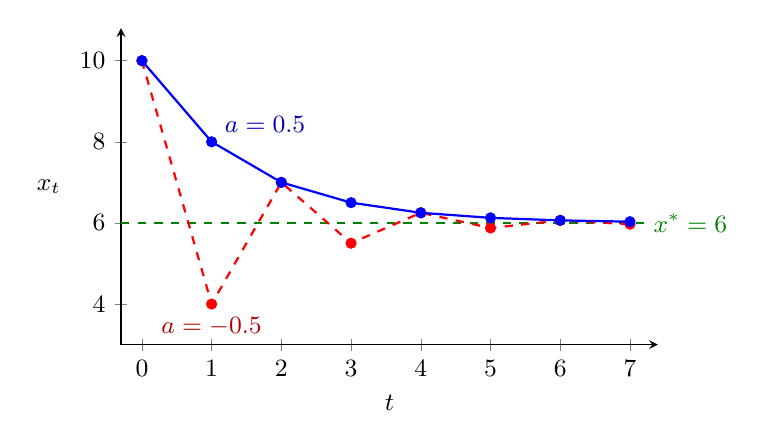
\begin{tikzpicture}[font=\small]
  \begin{axis}[
    axis lines=left, xmin=-0.3, xmax=7.4, ymin=3, ymax=10.8,
    xtick={0,1,...,7}, ytick={4,6,8,10}, xlabel={$t$}, ylabel={$x_t$}, ylabel style={rotate=-90},
    width=8.4cm, height=5.6cm, clip=false
    ]
    \addplot[green!50!black, thick, dashed, domain=-0.3:7.2] {6};
    \addplot[red, thick, dashed, mark=*, mark size=1.6pt, mark options={solid}, samples at={0,...,7}] {6+4*(-0.5)^x};
    \addplot[blue, thick, mark=*, mark size=1.6pt, samples at={0,...,7}] {6+4*0.5^x};
    \node[green!50!black, anchor=west] at (axis cs:7.2,6) {$x^*=6$};
    \node[blue!70!black, anchor=south west] at (axis cs:1.05,8) {$a=0.5$};
    \node[red!70!black, anchor=north] at (axis cs:1,3.9) {$a=-0.5$};
  \end{axis}
\end{tikzpicture}
\end{document}
